\section{Traje}
\label{sec:traje}

El primer paso del proyecto consistía en configurar el traje y poder usarlo dentro de Unity.
El traje usado, Preception Neuron 3, viene con:

\begin{enumerate}
	\renewcommand{\theenumi}{\alph{enumi}}
	\item 17 sensores identificados con cada punto.
	\item 15 Bandas de velcro que se ponen en el cuerpo para colocar los sensores.
	\item 3 puertos de carga para los sensores junto a 3 cables USB-C para conectarlos.
	\item 1 USB que contiene la licencia para poder conectar el traje al ordenador.
	\item 1 USB-C que funciona de receptor de las señales del traje.
\end{enumerate}

Para poder usar el traje se necesita la aplicación Axis Studio. \footnote{Enlace a la página de descarga de Axis Studio: \url{https://www.noitom.com/perception-neuron-downloads}}
\subsection{Axis Studio y conexión del traje}
Axis Studio es la aplicación creada por Noitom para poder capturar y grabar el movimiento en tiempo real y transmitirlo a aplicaciones de terceros (Unity, Blender o Unreal por ejemplo).

Mientras la aplicación está abierta es necesario tener el USB de la licencia introducido en el equipo.
Al abrir la aplicación y crear un proyecto aparece un espacio vacío (como se puede ver en la figura \ref{fig:AxisSinTraje}) en la parte izquierda de la pantalla, que es donde se verá en tiempo real la captación de movimiento; y un panel de la información del traje en la parte derecha.

\begin{figure}[H]
	\centering
	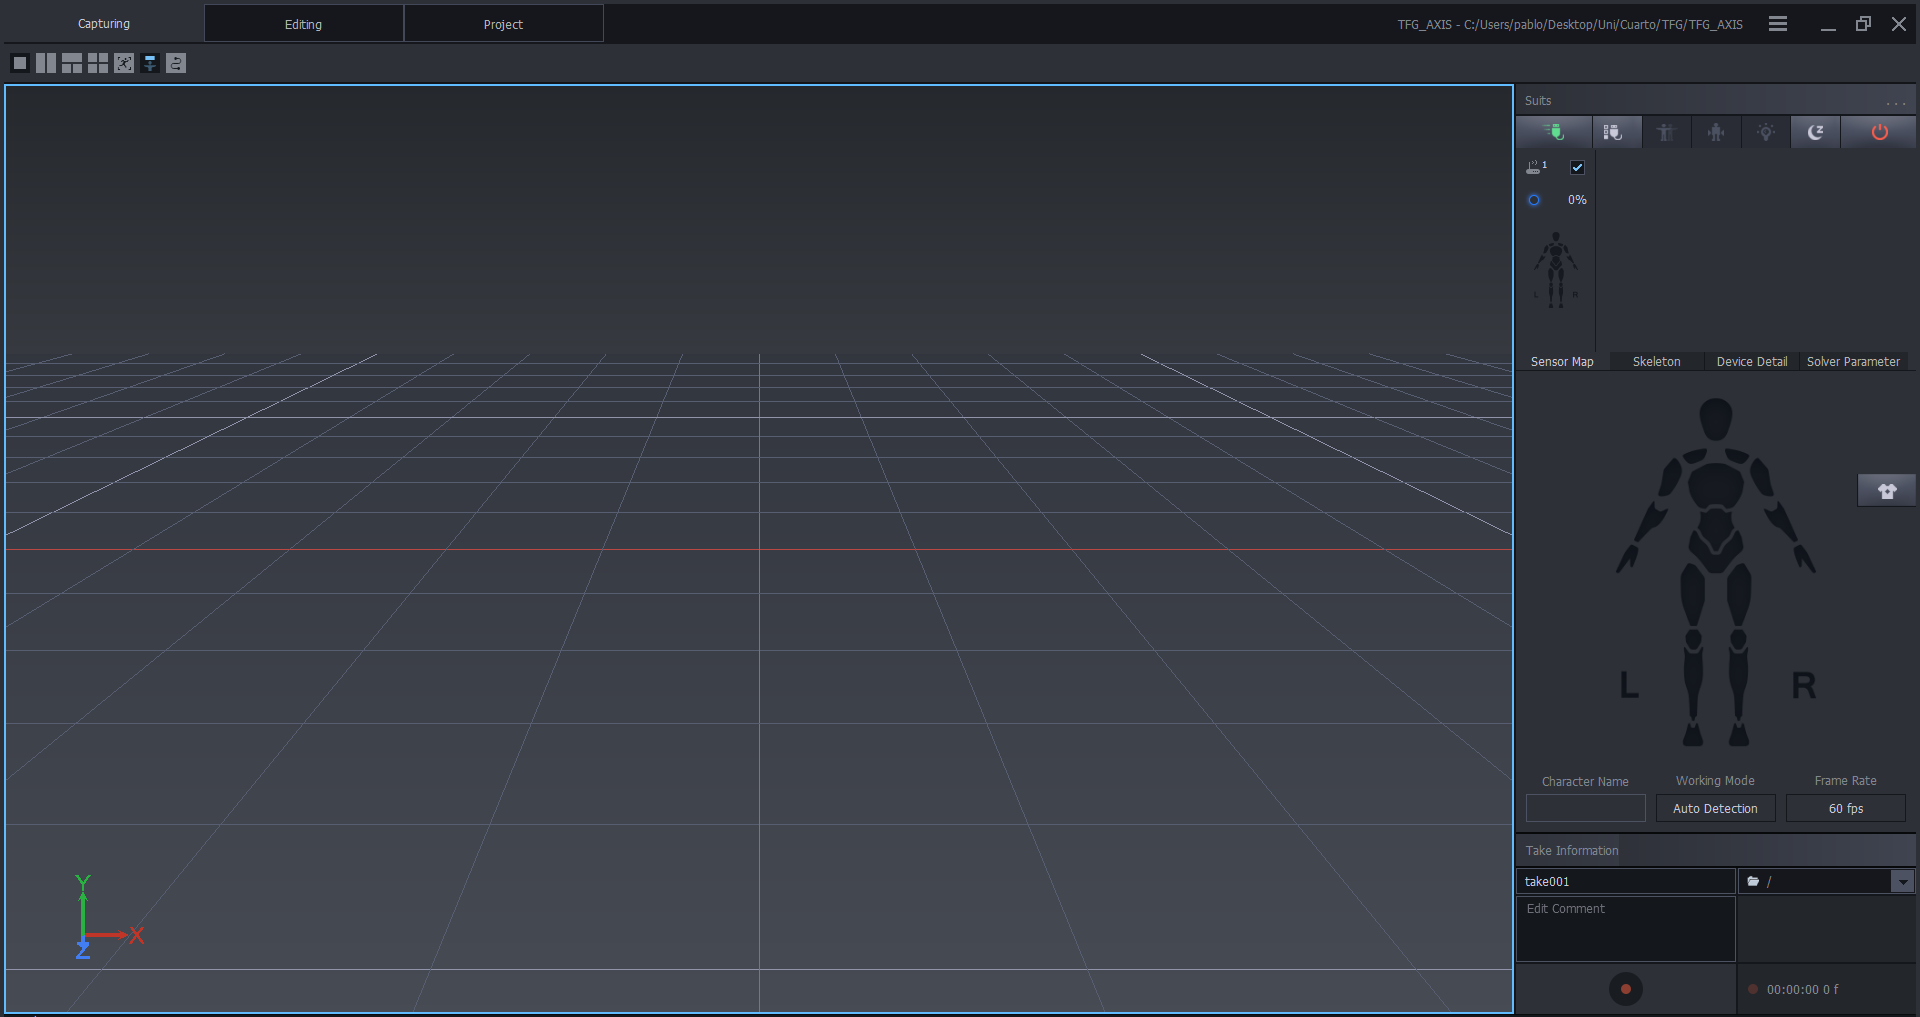
\includegraphics[width=0.5\textwidth]{Imagenes/Bitmap/AxisSinTraje.PNG}
	\caption{Captura de la aplicación Axis Studio antes de conectar un traje}
	\label{fig:AxisSinTraje}
\end{figure}

Para conectar el traje se debe tener enchufado en el mismo equipo el USB receptor y los puertos de carga con los sensores en ellos.
Posteriormente se deben desenchufar los puertos para que el traje se conecte con el receptor, que se muestra con un parpadeo azul en los sensores.

Una vez los sensores puestos en sus huecos de las bandas se debe pulsar al botón mostrado en la figura \ref{fig:BotonConectar} se debe calibrar el traje en el botón mostrado en la figura \ref{fig:BotonCalibrar}.
Esta calibración consiste en tres pasos:
\begin{enumerate}
	\item Posición de T: cabeza recta, piernas rectas paralelas a los hombros y brazos extendidos hacia los lados.
	\item Posición de S: cabeza recta, piernas ligeramente flexionadas, espalda recta y brazos extendidos hacia el frente.
	\item Posición de A: cabeza recta, piernas rectas paralelas a los hombros y brazos relajados paralelos al tronco.
\end{enumerate}

\begin{figure}[H]
	\centering
	
\includegraphics[width=0.5\textwidth]{Imagenes/Bitmap/ConectarTraje.PNG}
	\caption{Captura del botón para conectar el traje a Axis Studio}
	\label{fig:BotonConectar}
\end{figure}

\begin{figure}[H]
	\centering
	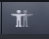
\includegraphics[width=0.5\textwidth]{Imagenes/Bitmap/Calibrar.PNG}
	\caption{Captura del botón para calibrar el traje}
	\label{fig:BotonCalibrar}
\end{figure}

Una vez el traje conectado y calibrado ya puede capturar el movimiento en tiempo real y transmitirlo a Unity.
\subsection{Unity y la conexión del traje}
\label{subsec:NeuronMocapLive}
Para poder usar la captura en Unity es necesario el plugin Neuron Mocap Live. \footnote{Enlace a la página de documentación de Neuron Mocap Live: \url{https://support.neuronmocap.com/hc/en-us/sections/206474008-UNITY-SDK}}

Una vez metido el plugin en el proyecto se necesita un objeto vacío que contenga el componente ``Neuron Source Manager''.
Este componente se conecta a la aplicación mediante la dirección IP de la máquina que ejecuta Axis Studio y sockets TCP a un puerto que puedes configurar en la aplicación de Axis Studio mediante el panel que se muestra en la figura \ref{fig:SettingAxis}

\begin{figure}[H]
	\centering
	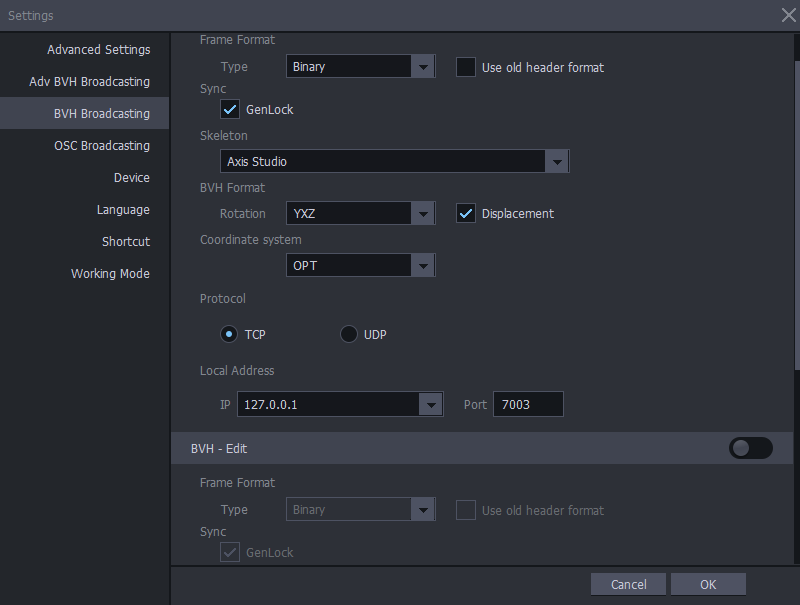
\includegraphics[width=0.5\textwidth]{Imagenes/Bitmap/SettingsAxis.PNG}
	\caption{Captura del panel de configuración de Axis Studio}
	\label{fig:SettingAxis}
\end{figure}

Posteriormente todos los objetos que vayan a usar la captura de movimiento deben ser hijos de este objeto vacío y tener el componente ``Neuron Transforms Instance''.
Este componente tiene una lista de Transforms que usa para mapear los huesos del traje con los del objeto de Unity.

\subsection{Limitaciones encontradas con el traje}
Durante el desarrollo del proyecto han habido dos limitaciones con respecto al traje.

La primera de ellos es la ausencia de guantes para capturar los dedos, ya que no vienen incluídos con el traje.
A pesar de que esto causa que los dedos estén siempre en la misma posición con respecto a la mano no ha causado ningún problema en la identificación de gestos

La segunda limiación es la cantidad de ruido electromagnético presente en nuestro espacio de trabajo: la Facultad de Informática de la Universidad Complutense de Madrid.
Este ruido causaba interferencias con el traje, haciendo que la señal con el ordenador fuese pobre constantemente y no se capturasen los movimientos correctamente.

Para solventarlo se requirió de un cable alargador de USB 2.0 de 10 metros que se conectaba al ordenador en el que se enchufaba el receptor y se acercaba lo más posible al traje, ampliando la señal al máximo.

Una vez conectado el traje, solventadas limitaciones y sabiendo los puntos que detecta era necesario un dataset que se puediera acoplar al esqueleto que proporciona el traje.